\section{Diagramme de séquence }

Nous avons choisi de proposer les diagrammes de séquence des parties les plus importantes de notre projet. 

\subsection{Inscription}
\begin{figure}[H]
  \center
  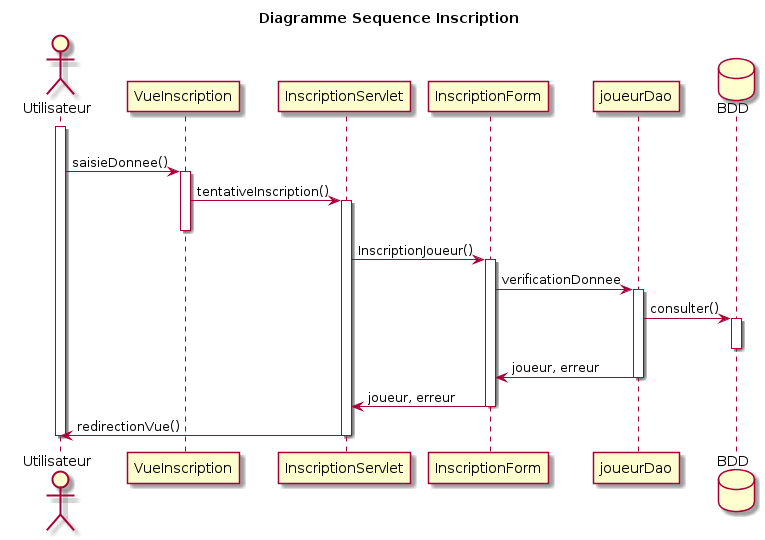
\includegraphics[scale=0.35]{../graph/DiagrammeSequenceInscription.png} \\
  \caption{Diagramme de séquence inscription}
\end{figure}

Ce diagramme correspond à l'inscription. L'inscription commence par la saisie du login et du mot de passe par l'utilisateur. Ensuite le formulaire d'inscription vérifie les données en entrée (login assez long et non utilisé, les deux mots de passe identiques). Si les données entrées sont correctes, l'utilisateur est alors ajouté à la base de donnée, avant d'ajouter le joueur dans la table on encrypte son mot de passe grâce à Jasypt. Si les données ne sont pas correctes, on renvoie un message d'erreur à l'utilisateur. 

\subsection{Connexion}
\begin{figure}[H]
  \center
  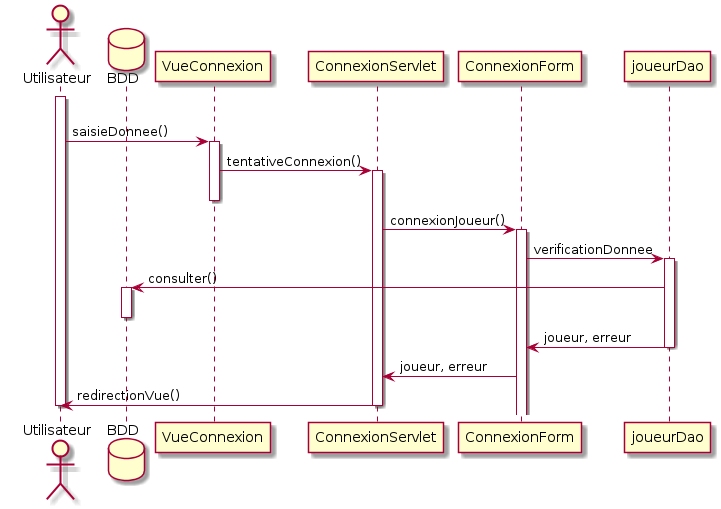
\includegraphics[scale=0.35]{../graph/DiagrammeSequenceConnexion.png} \\
  \caption{Diagramme de séquence connexion}
\end{figure}

Ce diagramme correspond à la connexion. Le principe est le même que pour l'inscription : le joueur saisie les données (login, mot de passe). Elles sont ensuite vérifiées par le formulaire de connexion. Si les données sont correctes le joueur est connecté et ajouté en session. L'utilisateur a ainsi accès a de nouvelles pages.

\subsection{Achat Actif}
\begin{figure}[H]
  \center
  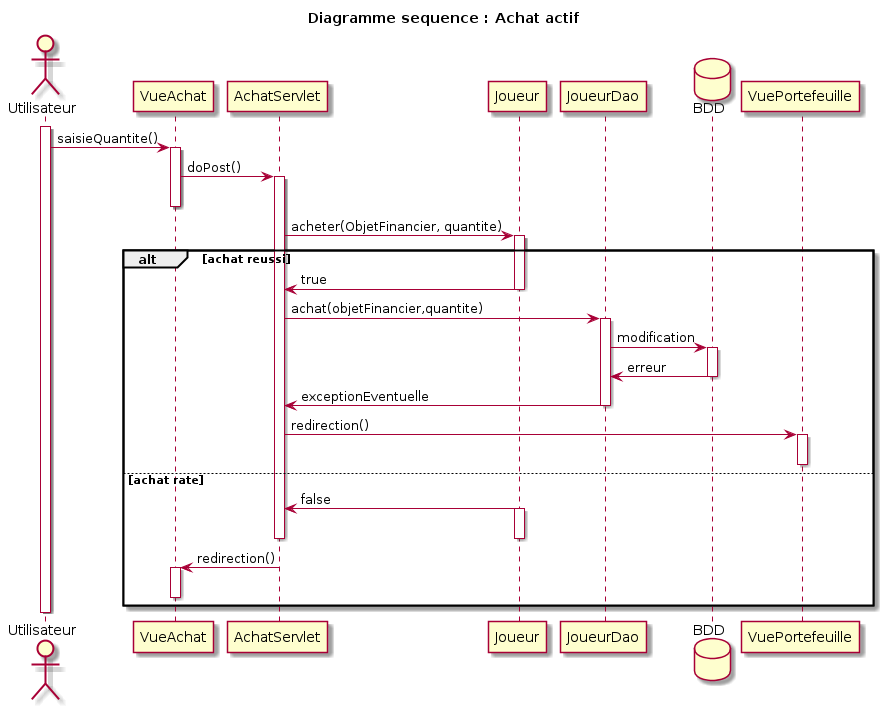
\includegraphics[scale=0.35]{../graph/DiagrammeSequenceAchatActif.png} \\
  \caption{Diagramme de séquence achat actif}
\end{figure}

Ce diagramme représente le diagramme de séquence général pour l'achat d'un objet financier. L'utilisateur choisit un actif qu'il veut acheter et choisit une quantité. Ensuit la servlet lance la méthode acheter du Joueur qui renvoie vraie si l'achat est réussi (argent disponible suffisant, quantité disponible de l'objet financier supérieur à la quantité demandée) et faux si l'achat échoue. Si l'achat est réussi on met à jour la base de donnée, s'il n'est pas réussi on renvoie un message d'erreur à l'utilisateur. 

\subsection{Achat Actif - Modele}
\begin{figure}[H]
  \center
  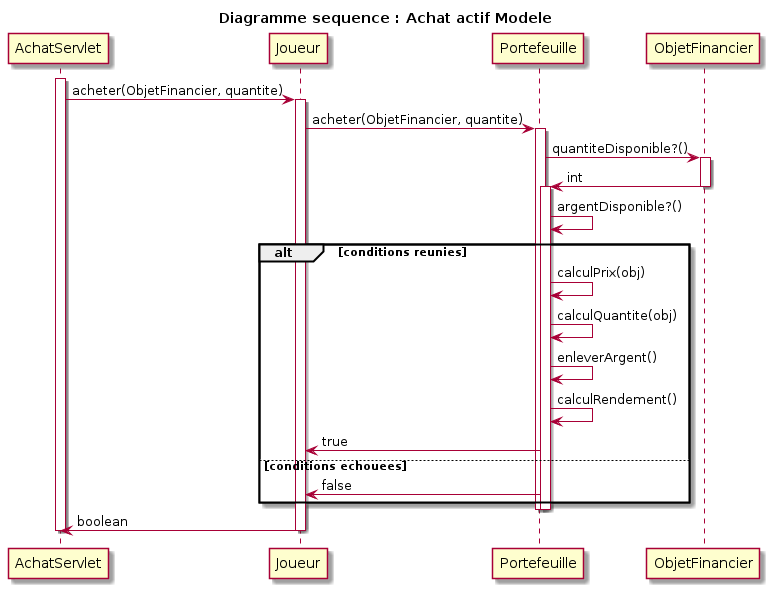
\includegraphics[scale=0.35]{../graph/DiagrammeSequenceAchatActifModele.png} \\
  \caption{Diagramme de séquence achat actif - Modele}
\end{figure}

Ce diagramme de séquence correspond à un zoom de ce qu'il se passe lors de l'achat d'un actif dans le modèle. Lors de l'achat d'un actif, le joueur appelle la méthode acheter du portefeuille. Le portefeuille vérifie d'abord que la quantité disponible est suffisante, ensuite que le joueur possède assez d'argent. Si les deux conditions précédentes sont réunies, on met à jour le prix de l'objet financier (moyenne pondéré avec l'ancien prix et les quantités), on met à jour la quantité de l'objet (simple addition) ainsi que l'argent disponible et le rendement du portefeuille. 

\subsection{Vente actif}
\begin{figure}[H]
  \center
  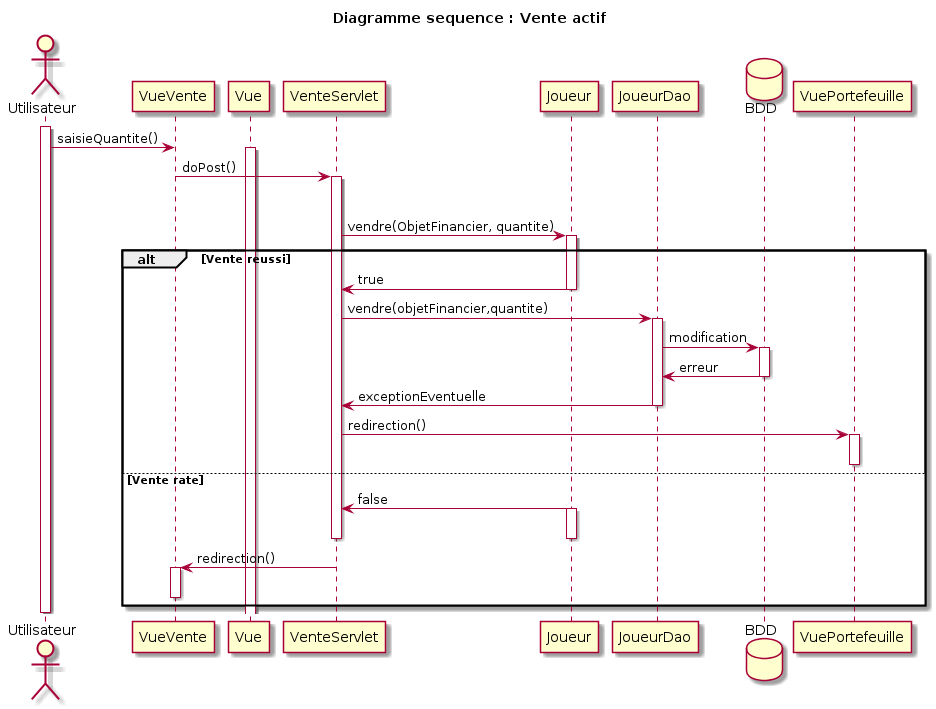
\includegraphics[scale=0.35]{../graph/DiagrammeSequenceVenteActif.png} \\
  \caption{Diagramme de séquence vente actif}
\end{figure}

Ce diagramme de séquence correspond au diagramme de séquence de la vente d'un actif. Le principe est le même que pour l'achat d'un actif c'est à dire que l'utilisateur choisit un actif et une quantité. On vérifie que la quantité d'actif que le joueur possède est supérieure à la quantité d'actifs qu'il souhaite vendre. Enfin, si c'est le cas on effectue la vente et on met à jour la base de données. Si ce n'est pas le cas, on lui renvoie un message d'erreur.  

\subsection{Supprimer portefeuille}
\begin{figure}[H]
  \center
  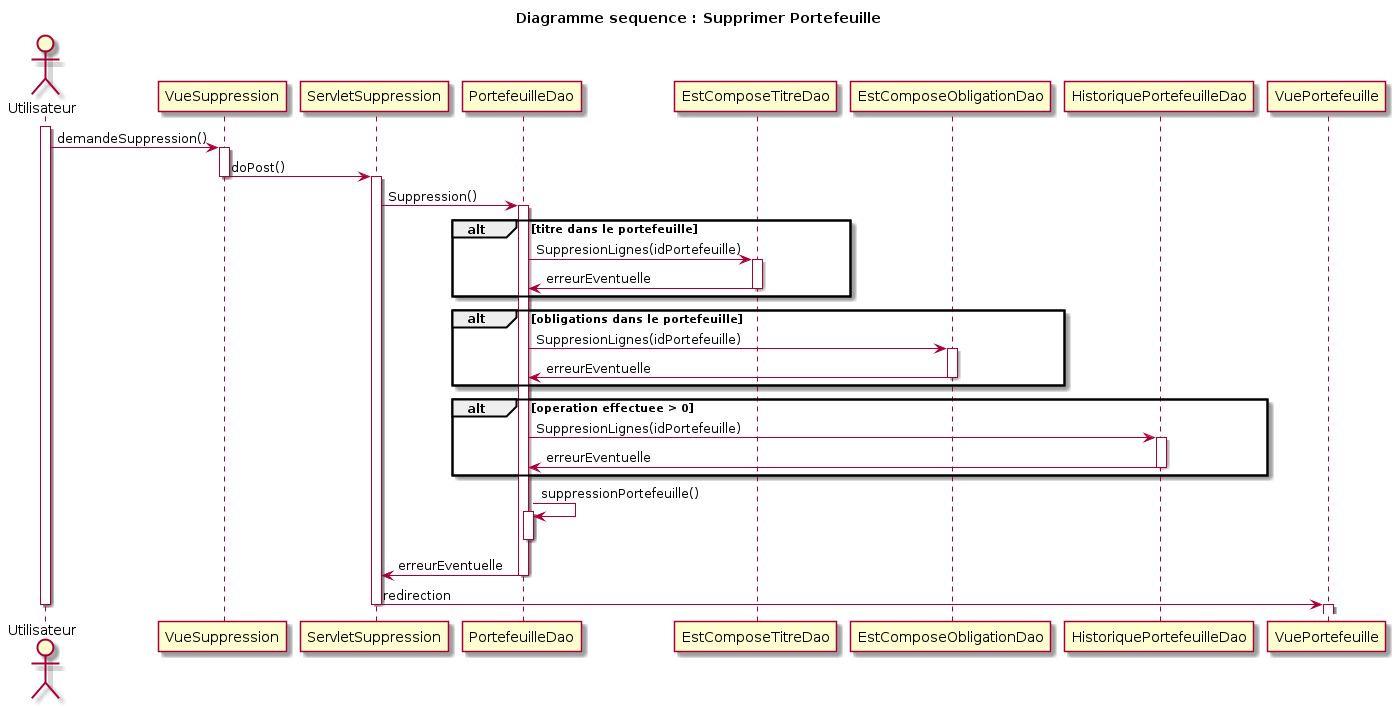
\includegraphics[scale=0.3]{../graph/DiagrammeSequenceSupprimerPortefeuille.png} \\
  \caption{Diagramme de séquence supprimer Portefeuille}
\end{figure}

La dernière opération principale que peut réaliser un joueur est la suppression de son portefeuille. Lors de la suppression du portefeuille, il faut supprimer toutes les lignes qui correspondent au portefeuille dans la base de données : il faut faire attention à l'ordre pour ne pas avoir de problèmes avec les clés lointaines. Nous supprimons donc d'abord les lignes dans EstComposeTitre et EstComposeObligation ensuite dans HistoriquePortefeuille qui correspond à l'historique des opérations et enfin dans la table Portefeuille. On attribue au joueur un nouveau portefeuille avec 10000 euros comme au début du jeu. 